\documentclass{standalone}
\usepackage{pgfplots}
\pgfplotsset{compat=1.17}
\begin{document}
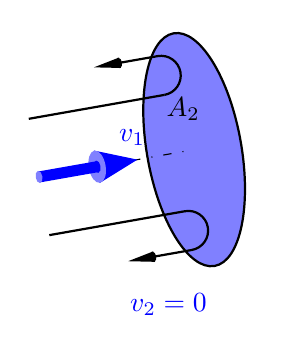
\begin{tikzpicture}[
bluedisc/.style={thick,fill=blue!20!white},
rest/.style={thick},
middleline/.style={loosely dash dot},
windarrow/.style={line width=4pt, blue}]

\begin{scope}[rotate=10]

\colorlet{bluedisc}{blue!20!white}
\colorlet{lightblue}{blue!50!white}

\draw[rest,fill=blue!50!white] (2,0) ellipse (.6 and 1.5);

\draw[middleline] (0,0) -- (2,0);

\begin{scope}[rest]
    \draw (0,0.75) -- (1.75,0.75);
    \draw (0,-0.75) -- (1.75,-0.75);
    \draw (1.75,-0.75) arc (90:-90:0.25) -- (1.25,-1.25);
    \draw (1.75,0.75) arc (-90:90:0.25) -- (1.25,1.25);
    \filldraw[black] (1,1.25) -- (1.25,1.3) -- (1.25,1.2) -- cycle;
    \filldraw[black] (1.25,1.25) ellipse (0.025 and 0.05);
    \filldraw[black] (1,-1.25) -- (1.25,-1.3) -- (1.25,-1.2) -- cycle;
    \filldraw[black] (1.25,-1.25) ellipse (0.025 and 0.05);
\end{scope}

\filldraw[blue] (1.25,0) -- (0.75,0.2) -- (0.75,-0.2) -- cycle;
    \filldraw[lightblue] (0.75,0) ellipse (.1 and .2);
    \draw[windarrow] (0,0) -- (0.75,0);
    \filldraw[lightblue] (0,0) ellipse (1pt and 2pt);
    \filldraw[blue] (0.75,0) ellipse (1pt and 2pt);
    \draw[windarrow] (0,0) (1.2,0) node[above] {$v_1$};

\draw (2,0.8) node[anchor=north] {$A_2$};

\draw[windarrow] (2,-2) node[anchor=east] {$v_2=0$};

\end{scope}
\end{tikzpicture}
\end{document}